\documentclass[journal=jpcbfk]{achemso}

\usepackage[version=3]{mhchem}
\usepackage[T1]{fontenc}
\newcommand*\mycommand[1]{\texttt{\emph{#1}}}
\newcommand{\todo}[1]{\textcolor{red}{#1}}

\usepackage{upgreek}				
\usepackage{xcolor}
\usepackage{booktabs}
\usepackage{multirow}
\usepackage{lmodern}
\usepackage{microtype}

\author{O. H. Samuli Ollila}
\email{samuli.ollila@helsinki.fi}
%\homepage[]{Your web page}
%\thanks{}
\affiliation{Research Program in Structural Biology and Biophysics, Insititute of Biotechnology, University of Helsinki}
\alsoaffiliation{Institute of Organic Chemistry and Biochemistry,
Czech Academy of Sciences, 
Prague 6, Czech Republic}

\author{Harri A. Heikkinen}
%\homepage[]{Your web page}
%\thanks{}
\affiliation{Research Program in Structural Biology and Biophysics, Insititute of Biotechnology, University of Helsinki}

\author{Hideo Iwa\"i}
%\homepage[]{Your web page}
%\thanks{}
\affiliation{Research Program in Structural Biology and Biophysics, Insititute of Biotechnology, University of Helsinki}



\SectionNumbersOn

\renewcommand{\thetable}{S\arabic{table}}%
\renewcommand{\thefigure}{S\arabic{figure}}%
\renewcommand{\thesection}{S\arabic{section}}%
\renewcommand{\thepage}{S\arabic{page}}%

\title{Supporting Information:\\Rotational Dynamics of Proteins from Spin Relaxation Times and Molecular Dynamics Simulations}

\begin{document}

\newpage
%\tableofcontents

\section{Mean square angle deviations of {\it Pa}TonB-96 simulated with tip4p water model}
\begin{figure*}[!h]
  \includegraphics[width=16.5cm]{../Figs/RMASDplotPsTonBtip4pT310K.eps}%
  \caption{Mean square angle deviations of inertia tensor axes calculated from {\it Pa}TonB-96
simulation with tip4p water model at 310K. The data shown with linear (left) and logarithmic scale
(right).  \label{RMASDplotLOG310}}%
\end{figure*}
\begin{figure*}[!h]
  \includegraphics[width=16.5cm]{../Figs/RMASDplotPsTonBtip4pT298K.eps}%                                                                                                    
  \caption{Mean square angle deviations of inertia tensor axes calculated from {\it Pa}TonB-96
simulation with tip4p water model at 298K. The data shown with linear (left) and logarithmic scale
(right).  \label{RMASDplotLOG310} \label{RMASDplotLOG298}}%                                                                                                                                                  
\end{figure*}

\newpage

\section{Accuracy of the scaling factors for rotational diffusion}
Accuracy of the spin relaxation calculations and scaling factors for rotational diffusion
were esimated by running three replicas of {\it Hp}TonB-92 and {\it Pa}TonB-96 simulations with tip3p.
In the first replica, the initial configuration was the lowest energy conformation from the NMR structure bundle.
In the second and third replicas, the starting configurations were randomly selected from the bundle.
Spin relaxation times calculated from the replicas are compared with the experimental data
in Figs. \ref{HpTonBrelaxationDATAreplicas} and \ref{PsTonBrelaxationDATAreplicas}.
\begin{figure*}[!b]
  \includegraphics[width=9cm]{../Figs/HpTonBrelaxationDATAreplicas.eps}%
  \caption{$^{15}$N spin relaxation times for {\it Hp}TonB-92 from experimental data (circles)
    and MD simulations with different initial configurations (squares). \label{HpTonBrelaxationDATAreplicas}}
\end{figure*}
\begin{figure*}[!h]
  \includegraphics[width=9cm]{../Figs/PsTonBrelaxationDATAreplicas.eps}%                                                                                                    
  \caption{$^{15}$N spin relaxation times for {\it Pa}TonB-96 from experimental data (circles)
    and MD simulations with different initial configurations (squares). \label{PsTonBrelaxationDATAreplicas}}
\end{figure*}

General agreement between the calculated spin relaxation times and experiments is essentially similar for all
the replicas of both proteins. Optimal scaling factors are also the same for different replicas, except for
the simulation1 of {\it Hp}TonB-92 which gives slightly lower scaling factor than the other two replicas.
Optimal values of the scaling factors for rotational diffusion from different simulations are summarized in
Table \ref{ROTdiffCOEFFSscaled}. The scaling factors for simulations with tip3p water model vary between 2.7--3.3, while
the scaling factors for simulations with tip4p, OPC4 and SPC/E water models are closer to 1.
The results are in line with the self-diffusion coefficients of water calculated from different water models \cite{izadi14},
also shown in Table \ref{ROTdiffCOEFFSscaled}.

\begin{table}[!h]
  \centering
  \caption{Scaling factors used to correct the overall rotational diffusion coefficients for different proteins
    simulated with different water models.
    $^{a}$ CMB64 protein from {\it Spirochaeta thermophila}
    $^{b}$ Calcium recoverin was 12 residues shorter in simulations than in experiments.
    $^{c}$ Ratio of isotropic rotational diffusion coefficients from simulations and experiments from Ref. \citenum{wong08}.
    $^{d}$ Ratio of simulated and experimental self-diffusion constant of water calculated from Ref. \citenum{izadi14}.  }\label{ROTdiffCOEFFSscaled}
  \begin{tabular}{c c c c c c c c c}
                                       &    & tip3p &  & tip4p && OPC4 && SPC/E \\
    \hline
    {\it Hp}TonB-92                    &    & 2.9 -- 3.3   &  & 1.0     && -  && - \\
    {\it Pa}TonB-96                    &    &  2.7    &  & 1.2   && -    && -\\
    {\it St}CBM64$^{a}$ \cite{heikkinen18}          &    &  -    &  & -     && 1.3  && -\\
    65K C-RRM \cite{norppa18}          &    & -     &  & 1.0     && -  && -\\
    Calcium recoverin$^{b}$ \cite{timr18}    &    &  3.2  &  & -     && -    && -\\
    &&&&&& \\
    GB3$^{c}$                           &    & -     &  & 1.1    && -   && 1.3 \\
    Ubiquitin$^{c}$                     &    & 2.7   &  & 1.1    && -   && 1.1 \\
    Binase$^{c}$                        &    & -     &  & -   && -   && 1.2 \\
    Lysosome$^{c}$                      &    & 2.7   &  & -    && -   && 1.3 \\
    &&&&&& \\
    Water self-diffusion$^{d}$  &    & 2.4   & & 1.1   &&  1 && 1.3 \\
    &&&&&& \\
  \end{tabular}
  \newline
  \flushleft
\end{table}

\pagebreak

\bibliography{refs.bib}

\end{document}
